\subsection*{Problema 17}

\textbf{Enunciado:} Evaluar la integral definida 
mediante sumas de Riemann usando las 
fórmulas de suma:
\begin{align*}
\int_{0}^{1} (x^2 - x^3) \, dx
\end{align*}

\textbf{Solución:} 

Utilizamos la definición de la integral 
definida como el límite de una suma de 
Riemann por la derecha. Dividimos el 
intervalo $[0, 1]$ en $n$ subintervalos de 
ancho igual a:
\begin{align*}
\Delta x = \dfrac{1 - 0}{n} = \dfrac{1}{n}
\end{align*}

Los puntos de muestreo son dados por 
$x_i = a + i \Delta x$:
\begin{align*}
x_i = \dfrac{i}{n}, \quad \text{para } i = 1, 2, \dots, n
\end{align*}

Evaluamos la función en cada punto $x_i$:
\begin{align*}
f(x_i) &= x_i^2 - x_i^3 \\
&= \left(\dfrac{i}{n}\right)^2 - 
\left(\dfrac{i}{n}\right)^3 \\
&= \dfrac{i^2}{n^2} - \dfrac{i^3}{n^3}
\end{align*}

Planteamos la suma de Riemann:
\begin{align*}
S_n &= \sum_{i=1}^{n} f(x_i) \Delta x \\
&= \sum_{i=1}^{n} \left( \dfrac{i^2}{n^2} - 
\dfrac{i^3}{n^3} \right) \dfrac{1}{n} \\
&= \dfrac{1}{n^3} \sum_{i=1}^{n} i^2 - 
\dfrac{1}{n^4} \sum_{i=1}^{n} i^3
\end{align*}

Aplicamos las fórmulas de sumas notables 
conocidas para cuadrados y cubos:
\begin{align*}
\sum_{i=1}^{n} i^2 &= \dfrac{n(n+1)(2n+1)}{6} \\
\sum_{i=1}^{n} i^3 &= \left[\dfrac{n(n+1)}{2}\right]^2
\end{align*}

Sustituimos estas fórmulas en la expresión 
de $S_n$:
\begin{align*}
S_n &= \dfrac{1}{n^3} \left[ \dfrac{n(n+1)(2n+1)}{6} \right] \\
&\quad - \dfrac{1}{n^4} \left[ \dfrac{n^2(n+1)^2}{4} \right]
\end{align*}

Simplificamos cada término algebraicamente:
\begin{align*}
S_n &= \dfrac{2n^3 + 3n^2 + n}{6n^3} - 
\dfrac{n^2 + 2n + 1}{4n^2} \\
&= \left(\dfrac{1}{3} + \dfrac{1}{2n} + 
\dfrac{1}{6n^2}\right) \\
&\quad - \left(\dfrac{1}{4} + \dfrac{1}{2n} + 
\dfrac{1}{4n^2}\right)
\end{align*}

Calculamos el límite cuando $n \to \infty$ 
para obtener el valor exacto de la integral:
\begin{align*}
\int_{0}^{1} (x^2 - x^3) \, dx &= \lim_{n \to \infty} S_n \\
&= \lim_{n \to \infty} \left[ \dfrac{1}{3} - 
\dfrac{1}{4} + \text{términos con } n \right] \\
&= \dfrac{1}{3} - \dfrac{1}{4} \\
&= \dfrac{4 - 3}{12} = \dfrac{1}{12}
\end{align*}

El valor de la integral definida es $\dfrac{1}{12}$.

\begin{figure}[H]
	\centering
	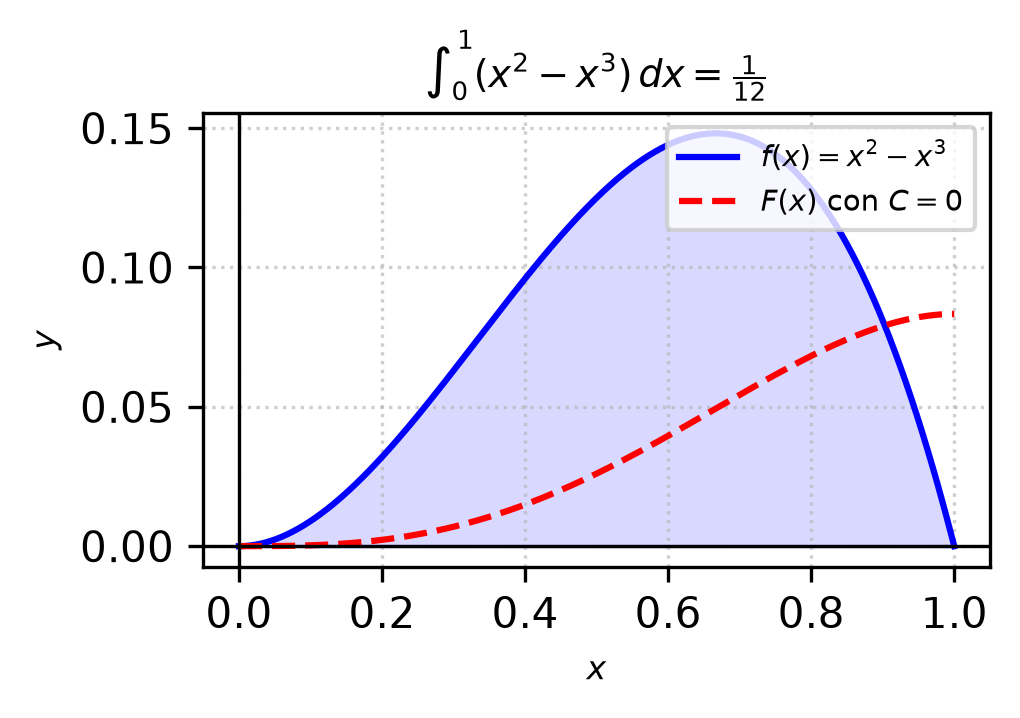
\includegraphics[width=\columnwidth]{semana_06/graficas/SEM06_P17_grafica.png}
	\caption{Representación gráfica de $f(x)$ y su antiderivada $F(x)$ evaluada para la constante de integración $C = 0$ (Problema 17).}
	\label{fig:problema17}
\end{figure}
